\chapter{State of the art}

\section{Titolo section}
Nel primo canto dell'Inferno, il pellegrino Dante si trova nella famigerata "selva oscura", che è simbolo esplicito di una situazione di traviamento esistenziale e spirituale che, per sua stessa ammissione, rischia di condurlo alle soglie della morte. L'aver scorto un colle rischiarato dalla luce divina non è che il primo passo del suo percorso di redenzione; le tre fiere che gli ostacolano il passo (la lonza, il leone, la lupa) lo costringono ad un lungo excursus nelle viscere infernali, durante il quale Dante sarà guidato da un altro "poeta" (v. 73), il buon Virgilio, che diverrà la sua guida morale e letteraria, subito dopo aver pronunciato la celebre profezia sul "veltro" (v. 101) che libererà il mondo terreno dal male e dal peccato \cite{lindskoog1986first}.

\begin{figure}[]
	\centering
	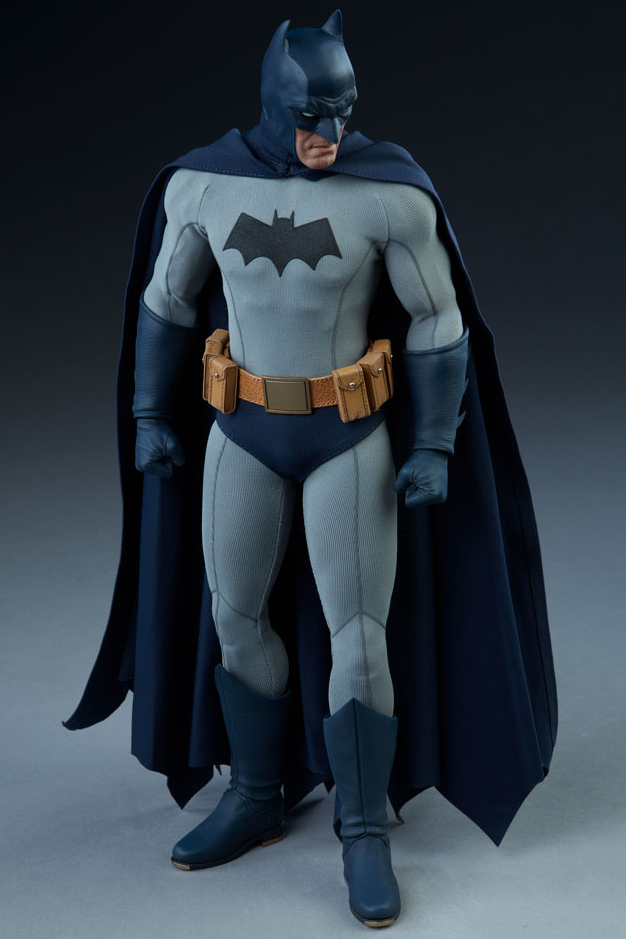
\includegraphics[width=.25\columnwidth]{images/batman}
	
	\caption{\textit{Just a Batman picture.}}
	\label{img:batman}
\end{figure}

\subsection{Titolo subsection}

Al di là dell'evidente e marcata metafora cristiana (il sacrificio e il martirio come testimonianza...), questa pellicola che ha tra i suoi protagonisti una Tilda Swinton strepitosa e sensualissima nel ruolo della malvagia strega, è visivamente seducente. Il luogo dominato da un eterno inverno, gli esseri fantastici e gli animali parlanti trasportano lo spettatore in un luogo di sogno dove anche i bambini protagonisti della pellicola in dinamiche sospese tra il gioco e l'eroismo personale \ref{img:batman}.


